\section{Further Insights}%
\label{sec:discussion}


\begin{figure}
\centering
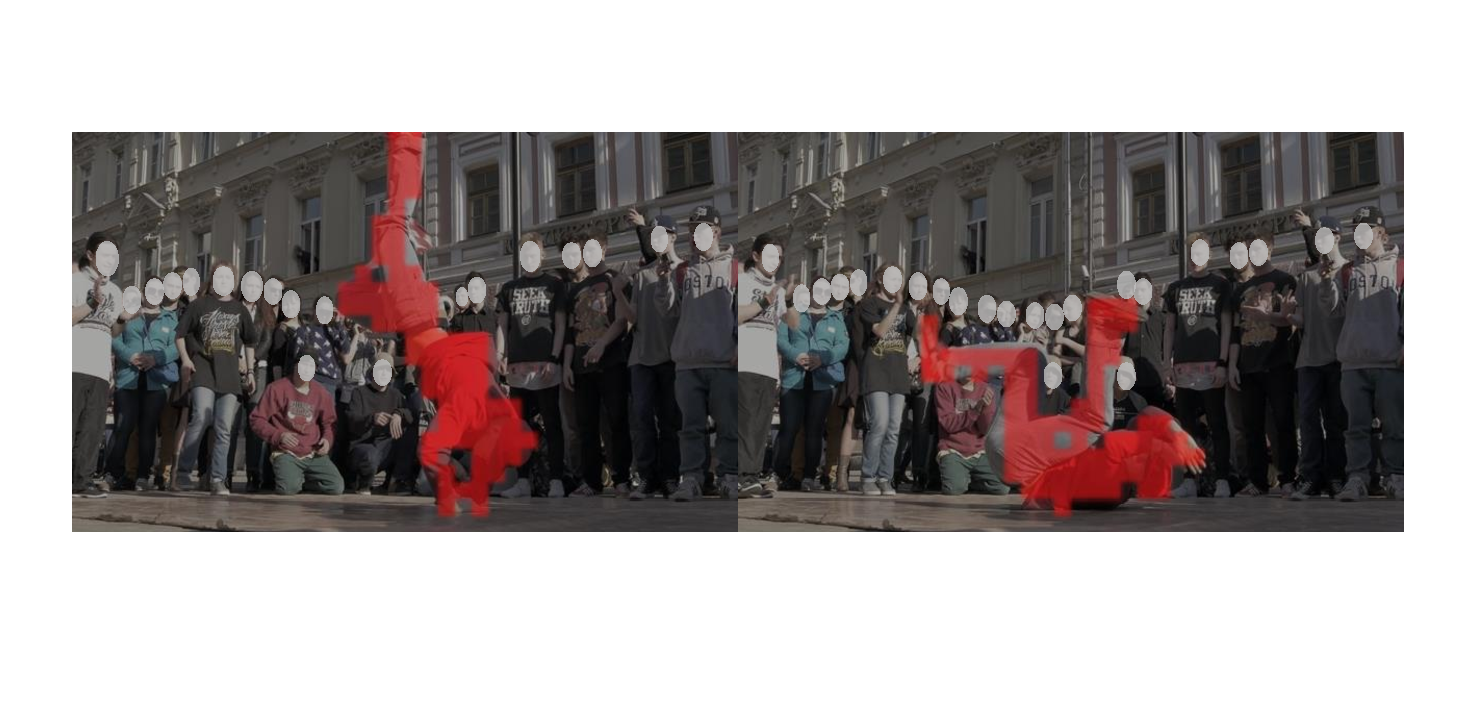
\includegraphics[width=0.95\linewidth]{figures/motion.pdf}
\caption{\textbf{Motion-Aware Representations.}
We cluster PCA-reduced intermediate image tokens by $k$-means and observe that the resulting clusters consistently separate the moving dancer from the static crowd and background, with red indicating high-response regions.
This suggests that \method learns motion-aware representations from reconstruction training, without explicit motion supervision.
}%
\label{fig:motion}
\end{figure}





As we developed \method, we made several empirical observations that are not yet rigorously established but that we think are still useful to share with other researchers interested in developing similar models.

\paragraph{Model Souping: Where Is the Information Stored?}

To better understand the model's behavior, we use model souping~\cite{wortsman22model} as a probe.
Specifically, we fuse the public VGGT checkpoint into \method by directly averaging specific subsets of their weights, without any further training.
Perhaps surprisingly, although the two models use different architectures (\eg, VGGT uses DINOv2 with a patch size of 14, whereas \method uses DINOv3 with a patch size of 16 and register attention), the averaged models can still produce visually reasonable reconstructions.

By fusing different subsets of the weights, we can gain insights into where different types of information are stored in the model.
Our first observation is that depth and field-of-view information is largely stored in the FFNs of the attention blocks, primarily in the frame-wise attention blocks and, to a lesser extent, in the global attention blocks.
This is consistent with the observations in the language community~\cite{geva21transformer,dai22knowledge,meng22locating}.
For example, as discussed in~\cref{sec:data_quality}, the model can memorize idiosyncratic noisy signals in the training data, such as treating humans as part of the ground in certain scenarios.
When we fuse the FFN weights of VGGT's frame-wise attention blocks into \method with a 50\%-50\% average, these errors are resolved.
In contrast, fusing the Q/K/V projection weights does not produce the same effect.
Camera extrinsic information appears to be encoded at a higher level and is not controlled solely by the FFN weights.
Finally, the ability to generalize to a variable number of input frames is also closely related to the frame-wise attention blocks.


\paragraph{Motion Awareness.}

Since the model can reconstruct dynamic sequences with large non-camera motion, we ask whether it learns to localize the moving regions.
To this end, we analyze the feature distributions of its intermediate tokens.
Specifically, we normalize intermediate image tokens across space and time, reduce their dimensionality with PCA, and group them using $k$-means.
No labels, optical flow, or learned probes are used at any stage.

As shown in \cref{fig:motion}, one PCA cluster consistently tracks the moving dancer across all frames while the static crowd and background remain in the other clusters.
This suggests that the ability to discriminate motion emerges automatically as a byproduct of the reconstruction objective, without explicit motion supervision.
Note also that the model is never given the temporal order of the input frames, either during training or inference.

We further examine how this signal evolves across layers.
Early layers (\eg, layer 4 in \cref{fig:motion}) produce the cleanest motion segmentation, isolating the dancer with minimal background response.
Middle layers, such as layer 13, retain a weaker but still discernible motion signal.
At the deepest layers (\eg, layer 23), the same clustering procedure highlights all people in the scene, indicating that the representations become increasingly global and semantic.

\paragraph{Normalizing Predictions.}

In VGGT, we discussed whether predictions should be normalized online to a unit coordinate space.
We further analyze this question here.
Consistent with the observation in VGGT, once the model has converged, we observe no difference in quantitative performance between training with and without prediction normalization.
The main benefit of normalization is qualitative: the final point clouds appear more spatially well spread. 
The drawback is that the optimization becomes less stable, with a steeper learning curve and a greater need for careful hyperparameter tuning to avoid gradient explosion.
If prediction normalization is necessary, we suggest initializing from a pretrained model to stabilize training, as in PI3.

\paragraph{DINO Initialization.}

As discussed above, \method is initialized from DINOv3.
We examined this choice and found that, without DINO initialization (\ie, from scratch), the model can still converge to similar performance, but requires 4--8$\times$ more training iterations.
DINOv3 substantially eases optimization and improves training efficiency.

\paragraph{Invalid Area Prediction.}

We experimented with an additional branch for predicting invalid regions, as in~\cite{wang24moge:, keetha26mapanything:}, with the hope that it would help the model ignore regions such as sky and prevent sky pixels from sticking to foreground objects in the point cloud.
Although the model predicted the invalid masks accurately, sky pixels still appeared in the foreground of the depth estimates, likely due to the lack of supervisory signals in these regions.
Therefore, in line with the idea of using as few dense heads as possible, we did not include this predictor in our final model.

\paragraph{Register Attention Only.}

We also tested using register attention only, without any full global attention.
In this setting, image tokens in one frame can never attend to image tokens in other frames.
All the inter-frame information exchange relies on registers instead.
Although this design reduces FLOPs to 6\% of the original model, performance drops to the level of the original VGGT\@.
This trade-off may be worth exploring for on-device applications.

\paragraph{Auxiliary Inputs.}

Theoretically, incorporating auxiliary inputs, such as temporal order, camera parameters, depth maps, or scale factors, can further enhance performance.
However, we empirically observe that introducing these priors during pretraining, even when applied randomly or masked across training iterations, is often detrimental.
Conversely, our preliminary experiments indicate that providing conditional auxiliary inputs exclusively during the fine-tuning phase is highly effective, improving task-specific performance without compromising the integrity of the learned representations.
While a comprehensive exploration is beyond the scope of this paper, we believe this represents a promising direction for future research.

\paragraph{Synthetic and Real Data Mixture.}

Consistent with the observations in VGGT~\cite{wang25vggt}, we find that synthetic and real data play complementary roles during training.
At a high level, although this distinction is not exact, synthetic data contributes more directly to accuracy, while real data improves generalization.
The main role of real data is to adapt the model to real-world appearance and expose it to more diverse camera trajectories.
In practice, we recommend sampling roughly 80\% synthetic data and 20\% real data in each epoch.
If sufficiently clean synthetic annotations are available, \eg after addressing the issues discussed in~\cref{sec:data_quality}, increasing the synthetic data ratio to around 90\% may be even better.

\paragraph{How to fine-tune VGGT/\method.}

When fine-tuning VGGT/\method for reconstruction tasks in a new data domain, we recommend two practical choices.
First, it is best to use a full learning-rate schedule, \ie, linear warm-up followed by cosine decay.
The peak learning rate should remain small, and the number of iterations need not be large, but completing the full schedule is typically preferable to using a constant learning rate.
Second, we found that the aleatoric uncertainty (confidence) loss can be unstable during fine-tuning.
We therefore recommend initially removing this loss, particularly when the fine-tuning dataset is very small.
If the downstream task requires confidence estimates, the uncertainty head can be fine-tuned separately.
When fine-tuning VGGT/\method for tasks besides reconstruction, we suggest increasing the warm-up ratio, \eg from 5\% to 10--15\%, and use a full scheduling cycle.


\paragraph{Self-Supervised Training.} 
In principle, self-supervised training is a powerful tool to scale training data.
So far, we have found it useful for improving model generalization, especially for out-of-distribution data, however, it has had little impact on most benchmarks.
It is non-trivial to do better.
Concurrent work has made a similar observation~\cite{huang2026self}. 
We spent considerable time exploring other self-supervised protocols such as new view synthesis, including variants similar to RayZer~\cite{jiang25rayzer:} and E-RayZer~\cite{zhao26e-rayzer:}, generating tokens instead of pixels, NeRF representations~\cite{barron21mip-nerf:} or Gaussian Splats~\cite{kerbl233d-gaussian}. 
We also tried masking image tokens, distinguishing objects across frames, incorporating temporal order, and related variants. 
Only the student-teacher approach helped, in our implementation. 
For example, we found methods like E-RayZer, which may work well with static scenes, struggle with dynamic ones.
This was counterintuitive to us, because much of self-supervised training in 2D relies on some form of \textit{invariance} (\eg, image augmentation in DINO), and reconstruction should naturally encode such invariance.  
We expected self-supervised reconstruction to work from scratch, whereas our successful approach still requires a pretrained model. 
Therefore, although the teacher-student self-supervised training in~\cref{sec:self-supervised-training} is not necessary to achieve our benchmark results, we still share it with the community, even though it makes our training pipeline look more complicated. 
Self-supervised reconstruction remains an open problem for the community. 
It may ultimately need to be integrated into a unified or omni-style model, as we discuss later. 




\paragraph{Dense Prediction Heads.}

In principle, strong latent representations should allow dense prediction tasks to be decoded with MLPs alone, without relying on convolutional layers, as evidenced by recent results such as JiT~\cite{li26back} or LagerNVS~\cite{szymanowicz26lagernvs}.
We explored this idea for a time because it aligned with our goal of keeping the framework as simple and scalable as possible.
However, we found that MLP-only heads consistently produced visible patch/block artifacts in the predicted depth maps, although they were often better than convolution-based alternatives in quantitative metrics, were much faster and more memory-efficient, and provided more stable gradients during training.
These artifacts are especially noticeable to humans, as they introduce geometric discontinuities that would otherwise be smooth.
We tried several remedies, including mipmap-style supervision~\cite{barron21mip-nerf:} (introducing local depth variance), probabilistic modeling (estimating depth with a probabilistic mixture of various independent channels),  and related variants, but they did not reliably remove the artifacts. 
Interestingly, the problem was much more prevalent in outdoor scenes than in indoor scenes, especially when the scene contained distant objects.
We suspect that this behavior is related to the numerical distribution of the prediction target.
For image generation tasks as studied by JiT, the output lies in a well-bounded numerical space.
In contrast, the range of geometric quantities, such as depth, is effectively unbounded.
This has motivated our trade-off, where we maintain a small number of convolutional layers followed by MLP layers.
The shallow convolutions operate at low feature resolutions, such as $16\times16$ or $32\times32$, and introduce little computational overhead, while accounting for most of the observed improvement in spatial smoothness. 
Notably, we used the shallow layers of DPT to keep the architecture comparable to prior methods, but any feature-pyramid-style convolution architecture can address the patch-artifact problem. 
Although we use the trade-off for \method, we still believe that MLP-only dense decoding heads are a promising and important direction for future exploration.

\section{Discussion}%
\label{sec:option}

We now discuss some decisions in designing \method, which are in part motivated by how we think feed-forward models can be most beneficial to the community.

\paragraph{Prioritizing Simplicity.}

We identified several architectural modifications that can further improve performance.
For example, while our model predicts the camera parameters in a single pass, better results can be obtained by using the iterative refinement design of the original VGGT~\cite{wang25vggt}.
The depth output can also be improved by injecting raw RGB values into the dense prediction head.
Using these and other techniques, we observed further improvements of 4\%--6\% in AUC@$3^\circ$ and about 2\% in \(\delta_{1.25}\) across multiple datasets, and we expect that further task-specific modifications can yield even more gains.
Even so, we deliberately decided to prioritize the overall simplicity of the model and the quality of the representation extracted by the feature backbone (aggregator). 
This choice is motivated by our observation that, once the backbone is well-trained, training a new or improved prediction head typically requires only 5--10K iterations.
Additionally, maintaining the simplicity of the architecture yields a cleaner base model, which we expect will be easier for the community to build upon.




\paragraph{Benefits of Feed-forward Reconstruction.}

Compared to traditional reconstruction pipelines, feed-forward reconstruction has three important advantages:
(a) efficiency,
(b) robustness, and
(c) representational power.
First, it is substantially faster, from tens to hundreds of times in some settings, and the gap can become even larger by streaming or by using multiple GPUs in parallel.
Second, it is much more robust than methods that rely heavily on explicit geometry optimization, like bundle adjustment.
For example, it can handle cases with little or no parallax, which are difficult to handle with triangulation-based methods.
Feed-forward reconstruction also readily extends to processing dynamic scenes, as shown in our experiments. 
Third, and perhaps most importantly, feed-forward reconstruction can extract versatile geometry-aware representations.
3D vision lacks powerful off-the-shelf general-purpose feature extractors comparable to the older VGG16~\cite{simonyan15very} or ResNet~\cite{he16deep} for 2D vision, let alone to modern 2D vision or vision-language foundation models.
As we show with several examples in this paper, feed-forward reconstruction is a promising proxy task for learning such a representation for 3D tasks.

Optimization-based reconstruction methods like COLMAP~\cite{schonberger16structure-from-motion} still have their strengths.
In well-conditioned settings, bundle adjustment can estimate the camera parameters to extremely high precision, reducing angular errors to a few hundredths of a degree.
Such accuracy remains valuable for applications like novel view synthesis with NeRFs~\cite{mildenhall20nerf:} or Gaussian splatting~\cite{kerbl233d-gaussian}.
Feed-forward reconstruction is not in conflict with optimization, instead, it can serve as a strong initialization for subsequent optimization procedures such as bundle adjustment.
Even so, given the rapid progress of feed-forward reconstruction in the short time since VGGT was introduced, we remain optimistic about future accuracy improvements and the applicability of this paradigm.

\paragraph{The Role of 3D/4D in the Era of Large Models.}

Spatial understanding is an area of increasing interest in vision-language, vision-language-action, vision-action, and world models~\cite{
chen24spatialvlm:,cheng24spatialrgpt:,zitkovich23rt-2:,cai26depthlm:,kim25openvla:,
team25gemini,hu23gaia-1:,li26causal,parker-holder25genie,nvidia25cosmos}. 
This is a natural consequence of developing embodied agents that operate in the physical world, which is three-dimensional.
In the short term, reconstruction models can be used as external tools to obtain explicit 3D information, such as depth and camera parameters.  
% 
They can also provide `structured' tokens that encode spatial information implicitly, as discussed in this paper. 
% 
In the long term, reconstruction might become a citizen in future unified models (`omni-model'), \ie, in large models pre-trained using multiple modalities, such as language and vision, and targeting multiple capabilities, such as understanding and generation~\cite{wang24emu3:,zhou25transfusion:,tong26beyond,team26longcat-next:,wang26ernie,team24chameleon:,wu25janus:,deng25emerging}. 
% 
This could be achieved by adding reconstruction-oriented data to model training without significant changes to the architecture or training framework. 
% 
For example, camera parameters can be predicted autoregressively as text, while pixel-wise quantities such as depth can be formulated as image generation, as recently explored in~\cite{yang26context}.



\paragraph{The next generation of reconstruction models, and perhaps more broadly perception systems, may be built on unified models.}
First, the biggest gain is likely to come from data, which is currently the main bottleneck for perception tasks like reconstruction.
Large-scale text and video corpora contain rich implicit descriptions of the physical world.
When geometry tasks are trained jointly with these modalities, they can tap into this massive, broader source of supervision.
Second, most perception problems are severely under-constrained when viewed in isolation.
A unified model naturally enforces cross-task consistency, allowing ambiguities in one domain (\eg, textureless regions in depth estimation) to be resolved by priors from another (\eg, semantic context).
Third, there is a paradigm-level reason to move in this direction: recent observations may indicate generative vision models scale more easily than perception-only vision models, and it seems generative models can transfer to perception to some extent~\cite{gabeur26image}.
We expect stronger, more robust perception models to emerge from multi-modal, multi-task training, rather than from reconstruction or perception objectives in isolation.
